% input files


\section*{Дифференцируемые отображения и криволинейные замены координат}

\sbsnum{4}{Дифференцируемые отображения и дифференицрование композиции}
\subsection{Обращение с обратным образом (?)}

На данный момент у нас есть отображения для $U \in \mathbb{R}^n$ и $V \in \mathbb{R}^k$, считая $U \overset{F}{\longrightarrow} V$

\vspace{-5mm}

\begin{minipage}[t]{0.45\textwidth}
\begin{align*}
    C^{\infty} (U) &\overset{F^*}{\longleftarrow} C^{\infty} (V) \\
    T_P U &\overset{d_P F}{\longrightarrow} T_{F(P)} V
\end{align*}
\end{minipage}
\hfill
\begin{minipage}[t]{0.45\textwidth}
\begin{align*}
    U &\overset{F}{\longrightarrow} V \overset{\varphi}{\to} \mathbb{R} \\
    U &\overset{F^* \varphi}{\longrightarrow} \mathbb{R},
    \hspace{0.5cm} 
    \text{где }
    \hspace{0.5cm} 
    F^* \varphi  \overset{\mathrm{def}}{=} \varphi \circ F,
\end{align*}
\end{minipage}

\vspace{-3mm}

\begin{equation}
    \overbrace{
        d_P F(
            \underbrace{X}_{\in T_P U}
            )
    }^{\in T_{F(P)} V}
    \underbrace{\varphi}_{\in C^{\infty} (V)} 
    =
    X 
    \underbrace{F^* \varphi}_{\in C^\infty (U)}.
\end{equation}

С формами ситуация схожая с функциями, то есть
$$
    C^\infty (V) = \Gamma^0 (V),
$$
получается
\begin{align*}
    \Omega^k (U) \overset{F^*}{\longleftarrow} \Omega^k (V), \\
    T_U U \overset{d_P F}{\longrightarrow} T_{F(P)} (V).
\end{align*}
Теперь пусть $X_1, \ldots, X_k$ -- векторное поле на $U$, тогда
$$
    (F^* \omega) (X_1, \ldots, X_k) = \omega\left(
        d F(X_1), \ldots, d F(X_k)
    \right).
$$
Собственно, факт:
\begin{equation}
    d F^* \omega = F^* \d \omega.
\end{equation}
И ещё факт
\begin{equation}
    F^* (\sigma \wedge \tau) = F^* \sigma \wedge F^* \tau.
\end{equation}



%%%%%%%%%%%%%%%%%%%%%%%%%%%%%%%%%%%%%%%%%%%%%%%%%%%%%%%%%%%%%%%%%%%%%%%%%%%%%%%%%%%
\subsection{Плоские кривые}
Кривые должны быть гладкими, но этого недостаточно. Поэтому требуем и \textit{регулярность}:
\begin{equation}
    \forall x, y \colon F(x, y) = 0
    \hspace{0.5cm} 
    \left(
        \frac{\partial F}{\partial x}, \frac{\partial F}{\partial y} 
    \right) \neq (0, 0),
\end{equation}
а в параметрическом задание
\begin{equation}
    \forall t \in (a, b)
    \hspace{0.5cm} 
    \dot{\vc{r}} (t) = (\dot{x} (t), \dot{y}(t)) \neq (0, 0).
\end{equation}

Пусть $F(x, y) = 0$ -- регулярная гладкая неявно заданная кривая. Тогда в окрестности любой своей точки её можно задать как регулярную гладкую параметрическую кривую. 





% \newpage 

\sbsnum{5}{Системы криволинейных координат и теорема об обратном отображении}
\subsection{Производная по направлению}

Раньше определили
$$
    \partial_V f(A) = \lim_{\varepsilon \to 0} \frac{f(A + \varepsilon V) - f(A)}{\varepsilon},
$$
но сложность в том, что $A + \varepsilon V \notin \Sigma$. 
Но гладкую функцию с поверхности может всегда продлить в некоторую окрестность поверхности. Это продолжение $F$ не единственно. 

\begin{to_def} 
    Определим
    $$
         \partial_V f(A) \overset{\mathrm{def}}{=} \partial_V F(A),
    $$ 
    при чём def инвариантно к выбору $F$.
\end{to_def}

\begin{proof}[$\triangle$]
    \begin{minipage}[t]{0.9\textwidth}
        \begin{enumerate}[label = \Roman*.]
            \item Мы дифференцируем только вдоль касательных векторов к $\Sigma$, следовательно существует кривая $\gamma$ на $\Sigma$ такая, что
            \begin{align*}
                &1) \ \forall t \; \gamma(t) \in \Sigma \\
                &2) \ \gamma(0) = A \\
                &3) \ \ddot{\gamma}(0) = V.
            \end{align*}
            \item Тогда
            $$
                \underbrace{\frac{d}{dt} f(\gamma(t)) \bigg|_{t=0}}_{
                *
                } = 
                \frac{d}{dt} F(\gamma(t)) \bigg|_{t=0} =
                \frac{\partial F}{\partial x^i} (\set{x}{n}) \dot{x}^i (t) \bigg|_{t=0} =
                \frac{\partial F}{\partial x^i} (A) V^i = 
                \underbrace{\partial_V F(A)}_{
                **
                }
                ,
            $$
            считая $\gamma(t) = [x^1(t),\ldots, x^n(t)]$.
            \item Но, т.к. $*$ не зависит от выбора $F$, то и $**$ не зависит от выбора $F$. Тогда $\partial_V f(A)$ определена корректно.
            \item К слову, $**$ не зависит от выбора пути, тогда и $*$ не зависит от выбора пути.
        \end{enumerate}
    \end{minipage}

\phantom{42}
\end{proof}

Получается мы можем определить понятие  дифференцирования гладкой функции на поверхности в точке.

\begin{to_def} 
     Для $f\colon \Sigma \to \mathbb{R}$ достаточно быть определенной в некоторой окрестности точки $A$. Скажем, что $D$ -- дифференцирование на $\Sigma$ в точке$A$, если
    \begin{align*}
        &1) \ Df \in \mathbb{R} \\
        &2) \ D(f+g) = Df + Dg \\
        &3) \ D(fg) = (Df) \cdot g(A) + f(A) \cdot (Dg).
    \end{align*}
    Пусть $\set{u}{k}$ -- локальные координаты в окрестности точки $A$.
\end{to_def}


\begin{to_lem} 
     Для $\forall D \ \exists \set{V}{K}$ такой, что
     $$
         Df = \frac{\partial f}{\partial u^i} (A) V^i.
     $$
\end{to_lem}

Пусть есть некоторый касательный вектор $W \in T_A \Sigma$
$$
    W = W^i r_{u^i} (A).
$$
Тогда можно рассматривать путь $\gamma(t)$ в локальных координатах такой, что
$
    \gamma(0) = A, \ \dot{\gamma}(0) = W,
$
то есть для $A = (\set{u_0}{k})$ и $\gamma(t) = \left[
    u^1(t), \ldots, u^k(t)
\right]$ верно, что
$$
    u^i(0) = u^i_0, \hspace{0.5cm} \dot{u}^i(0) = W^i.
$$
Тогда
$$
    \partial_W f(A) = \frac{d}{dt} f(\gamma(t)) \bigg|_{t=0}
    =
    \frac{\partial f}{\partial u^i} (A) \ W^i.
$$

Получается, что \textbf{каждый} касательный вектор $W$ даёт дифференцирование $\partial_W \big|_A$, и \textbf{каждое} дифференцирование в $A$ получается из касательного вектора. Поэтому будем писать просто
\begin{equation}
    \boxed{
    W = \partial_W = W^i \frac{\partial }{\partial u^i} .
    }
\end{equation}


\subsection{Двойственность}

Раз есть касательные векторы, то есть и кососимметрические полилинейные функии на них. 
Так приходим к следующей двойственной структуре:

$\cdot$ $T_P \Sigma$ -- \textit{касательное пространство} к $\Sigma$ в $P$,

$\cdot$ $T_P^* \Sigma \overset{\mathrm{def}}{=}  \left(T_P \Sigma\right)^*$ -- \textit{кокасательное пространство} к $\Sigma$ в $P$.

\noindent
Получаются векторное поле $X$: $X(P) \in T_P \Sigma$, и ковекторное поле $\xi$:
$\xi (P) \in T_P^* \Sigma$.

Если $\set{u}{k}$ -- локальные координаты на $\Sigma$, то
$$
    \frac{\partial }{\partial u^i} = r_{u^i}
    \hspace{0.5cm} \text{---} \hspace{0.5cm} 
    \text{базис в } T_P \Sigma.
$$
Соответственно,
$$
    du^1, \ldots, du^k
    \hspace{0.5cm} \text{---} \hspace{0.5cm} 
    \text{базис в } T_P^* \Sigma.
$$
А вот
$$
    \underset{ i_1 < \ldots < i_q}{ du^{i_1} \wedge \ldots \wedge du^{i_q}}
    \hspace{0.5cm} \text{---} \hspace{0.5cm} 
    \text{базис в } \Lambda^q T_P^* \Sigma,
$$
где $\Lambda^q T_P^* \Sigma$ -- пространство $q$-форм.




\sbsnum{6}{Теоремы о системе неявных функций}
\sbsnum{20}{Интегрирование диф-формы объёма}
Естественно ввести \textit{тензор электромагнитного поля}:
\begin{equation}
{F}_{ik} = 
    \begin{pmatrix}
        0    & E_x & E_y  & E_z   \\
        -E_x  & 0    & -B_z & B_y   \\
        -E_y & B_z  & 0    & -B_x  \\
        -E_z & -B_y & B_x & 0     \\
    \end{pmatrix}_{ik},
    \hspace{2cm} 
{F}^{ik} = 
    \begin{pmatrix}
        0    & -E_x & -E_y  & -E_z   \\
        E_x  & 0    & -B_z & B_y   \\
        E_y & B_z  & 0    & -B_x  \\
        E_z & -B_y & B_x & 0     \\
    \end{pmatrix}^{ik}
\end{equation}
Тогда уравнения Максвелла запишутся в виде
\begin{equation}
    \boxed{
        \varepsilon^{iklm} \partial_k F_{lm} = 0, \hspace{0.5cm} 
        \partial_k F^{ik} = - \frac{4\pi}{c} j^i
    },
\end{equation}
где $j^i = (\rho c, \vc{j})$. Прямой подстановкой тензора ЭМ поля нетрудно убедиться, что

\phantom{42}

\noindent
\begin{minipage}[t]{0.45\textwidth}
\noindent
Дифференциальная форма в СГС:
    \begin{align}
        \vphantom{\oint }
        \div \vc{D} &= 4 \pi \rho \\
        \vphantom{\oint }
        \div \vc{B} &= 0 \\
        \vphantom{\oint }
        \rot \vc{E} &= -\frac{1}{c} \frac{\partial \vc{B}}{\partial t}  \\
        \vphantom{\oint }
        \rot \vc{H} &= \frac{4\pi}{c} \vc{j} + \frac{1}{c} \frac{\partial \vc{D}}{\partial t} 
    \end{align}
\end{minipage}
\hfill
\begin{minipage}[t]{0.45\textwidth}
Интегральная форма в СГС:
    \begin{align}
       \oint \vc{D} \cdot d \vc{s} &= 4\pi Q \\
       \oint \vc{B} \cdot d \vc{s} &= 0 \\
       \oint \vc{E} \cdot d \vc{l} &= - \frac{1}{c} \frac{d}{dt} \int \vc{B} \cdot d \vc{s} \\
        \oint \vc{H} \cdot \d \vc{l} &= \frac{4\pi}{c} I + \frac{1}{c} \frac{d}{dt} \int \vc{D} \cdot \d \vc{s}.
    \end{align}
\end{minipage}

\begin{description*}
    \item[$\vc{E}$]  --- напряженность электрического поля;
    \item[$\vc{H}$]  --- напряженность магнитного поля;
    \item[$\vc{D}$]  --- электрическая индукция;
    \item[$\vc{B}$]  --- магнитная индукция.
\end{description*}

\subsubsection*{Материальные уравнения}

В проводниках связь между плотностью тока и напряжённостью электрического поля выражается в линейном приближении \textit{законом Ома}:
\begin{equation*}
    \vc{j} = \sigma \vc{E},
\end{equation*}
где $\sigma$ -- \textit{удельная проводимость среды}.

В среде сторонние электрические и магнитные поля вызывают поляризация $\vc{P}$ и намагничивание вещества $\vc{M}$.
Тогда
\begin{align*}
    \rho_\text{b} &= - \nabla \cdot \vc{P} \\
    \vc{j}_\text{b} &= c \nabla \times \vc{M} + \frac{\partial \vc{P}}{\partial t} ,
\end{align*}
Далее, по определению
\begin{align*}
    \vc{D} &= \vc{E} + 4\pi \vc{P}, &\vc{B} &= \vc{H} + 4 \pi \vc{M} \\
\end{align*}
Что в случае линейной поляризации или линейной намагничиваемости можно записать, как  
$$
    \left\{\begin{aligned}
        \vc{P} &= \chi_{\text{e}} \vc{E}, \\
        \vc{M} &= \chi_{\text{m}} \vc{H}, \\
    \end{aligned}\right.
    \hspace{0.5cm} \Rightarrow \hspace{0.5cm} 
    \left\{\begin{aligned}
         \vc{D} &= \varepsilon \vc{E} = (1 + 4\pi \chi_{\text{e}}) \vc{E}, \\
       \vc{B} &= \mu \vc{H} = (1 + 4 \pi \chi_{\text{m}}) \vc{H}.
    \end{aligned}\right.
$$
где $\varepsilon$ -- \textit{\sout{относительная} диэлектрическая проницаемость}, $\mu$  — \textit{относительная магнитная проницаемость}, $\chi_{\text{e}}$  -- \textit{диэлектрическая восприимчивость}, $\chi_{\text{m}}$ -- \textit{магнитная восприимчивость}.

Наконец, в однородных средах верно, что
\begin{equation*}
    \left\{\begin{aligned}
        \div \vc{E} &= 4\pi \frac{\rho}{\varepsilon},  \\
        \div \vc{B} &= 0,
    \end{aligned}\right.
    \hspace{1cm} 
    \left\{\begin{aligned}
        \rot \vc{E} &= - \frac{1}{c} \frac{\partial \vc{B}}{\partial t}, \\
        \rot \vc{B} &= \frac{4\pi}{c} \mu \vc{j} + \frac{\varepsilon \mu}{c} \frac{\partial \vc{E}}{\partial t},
    \end{aligned}\right.
\end{equation*}
где в оптическом диапазоне принято $n = \sqrt{\varepsilon \mu}$.

\subsubsection*{Граничные условия}
Опять же, в СГС,
\begin{equation*}
    \left\{\begin{aligned}
        (\vc{E}_1 - \vc{E}_2) \times \vc{n}_{1,2} &= 0, \\
        (\vc{H}_1 - \vc{H}_2) \times \vc{n}_{1,2} &= \frac{4\pi}{c} \vc{j}_\text{s},
    \end{aligned}\right.
    \hspace{1cm} 
    \left\{\begin{aligned}
        \left(\vc{D}_1 - \vc{D}_2\right) \cdot \vc{n}_{1,2} &= - 4\pi \rho_\text{s}, \\
        \left(\vc{B}_1 - \vc{B}_2\right) \cdot \vc{n}_{1, 2} &= 0,
    \end{aligned}\right.
\end{equation*}
где $\rho_{\text{s}}$ -- поверхностная плотность свободных зарядов, $\vc{j}_\text{s}$ -- плотность поверхностных свободных токов вдоль границы. 

Эти граничные условия показывают непрерывность нормальной компоненты вектора магнитной индукции, и непрерывность на границе областей тангенциальных компонент напряжённостей электрического поля. 

\subsubsection*{Уравнение непрерывности}

Источники полей $\rho, \vc{j}$ не могут быть заданы произвольным образом. Применяя операцию дивергенции к четвёртому уравнению (закон Ампера—Максвелла) и используя первое уравнение (закон Гаусса), получаем уравнение непрерывности
\begin{equation*}
    \nabla \cdot \vc{j} + \frac{\partial \rho}{\partial t} = 0,
    \hspace{0.5cm} \Leftrightarrow \hspace{0.5cm} 
    \oint_S \vc{j} \cdot \d \vc{s} = - \frac{d }{d t} \int_V \rho \d V.
\end{equation*}




\sbsnum{21}{Представление диф-формы в каноническом виде}
\begin{to_lem} 
\label{lem_6.100}
    Пусть $U = \prod_{i=1}^n (a_i, b_i)$, где $(a_i, b_i) \ni 0$. Пусть $\varphi \colon \mathbb{R} \mapsto \mathbb{R}^+$ -- гладкая функция с компактным носителем, содержащимся в каждом $(a_i, b_i)$, и с единичным интегралом. Для всякой $\nu \in \Omega_{\text{c}}^n (U)$ найдётся число $I$ и форма $\lambda \in \Omega_{\text{c}}^{n-1}(U)$, такие что
    $\nu = I \varphi(x_1) \ldots \varphi(x_n) dx_1 \wedge \cdots \wedge dx_n + d \lambda$.
\end{to_lem}


\begin{to_con} 
\label{con_6.101}
    Пусть $U = \prod_{i=1}^{n} (a_i, b_i)$ -- произведение интервалов. Факторпространство $\Omega_{\text{c}}^n(U) / d \Omega_{\text{c}}^{n-1} (U)$ одномерно. Получается, что всевозможные способы определить интеграл формы $\nu \in \Omega_{\text{c}}^n (U)$ так, чтобы интеграл от $d \lambda$ равнялся нулю, могут отличаться только умножением на константу. \red{Ещё раз.} 
\end{to_con}

\sbsnum{22}{Поведение интеграла от формы при линейной замене координат}

\begin{to_lem}[Поведение интеграла формы при линейной замене координат]
     Интеграл дифференциальной формы $\nu \in \Omega_{\text{c}}^n (\mathbb{R}^n)$ при отображении $A^*$, соответствующем линейному преобразованию $A : \mathbb{R}^n \mapsto  \mathbb{R}^n$ меняет или не меняет знак в зависимости от знака определителя $\det A$, то есть
     \begin{equation*}
         \int_{\mathbb{R}^n} A^* \nu = (\sign \det A) \int_{\mathbb{R}^n} \nu.
     \end{equation*}
\end{to_lem}


\sbsnum{23}{Гладкое разбиение единицы}
\subsubsection*{Давление света}
При полном поглощении запишем следующее:
\begin{equation*}
    w = \frac{E^2}{4\pi} = pc, \hspace{0.5cm} p = \frac{E^2}{4\pi c} 
    \hspace{0.5cm} \Rightarrow \hspace{0.5cm} 
    P = \frac{1}{dS} \frac{d (p\d V)}{d t} = \frac{E^2}{4\pi},
    \hspace{0.5cm} 
    \langle P\rangle = \frac{\langle E^2\rangle}{4\pi}.
\end{equation*}
Или, по-другому
\begin{equation*}
    \left\{\begin{aligned}
        \frac{\partial \vc{E}}{\partial z} &= \rot \vc{E} = - \frac{1}{c} \frac{\partial \vc{H}}{\partial t}, \\
        \frac{\partial \vc{H}}{\partial z} &= \rot \vc{H} = \frac{4\pi}{c} \vc{j} + \frac{1}{c} \frac{\partial E}{\partial t}.
    \end{aligned}\right.
    \hspace{0.5cm} \Rightarrow \hspace{0.5cm} 
    \frac{\partial }{\partial z} \left(\frac{E^2+H^2}{8\pi} \right) = - \frac{1}{c} \frac{\partial \vc{H}}{\partial t} \cdot \frac{\vc{E}}{4\pi}  + \frac{4\pi}{c} \vc{j} \cdot \frac{\vc{B}}{4\pi} + \frac{1}{c} \frac{\partial \vc{E}}{\partial t} \frac{\partial \vc{H}}{\partial 4\pi} = \vc{f} + \frac{1}{8\pi c} \frac{\partial }{\partial t} \left(\vc{E} \cdot \vc{H}\right).
\end{equation*}
Таким образом
\begin{equation*}
    \frac{\partial }{\partial z} 
    \vph
    \langle w\rangle= \langle f \rangle
    \hspace{0.5cm} \Rightarrow \hspace{0.5cm} 
    \langle P\rangle = \int_0^{\infty} \langle f\rangle\d z = w(0) - w(\infty) = w(0) = \frac{\langle E^2\rangle}{4\pi}.
\end{equation*}
Что и требовалось доказать!) Кстати,
\begin{equation*}
\overline{S} = c \cdot \overline{\mathcal W_{\text{эл}}}, \hspace{0.5cm} \Rightarrow \hspace{0.5cm} 
    \vc{g}_{\text{эм}} = \frac{1}{c^2} \vc{S} = \frac{1}{4\pi c} \left[
        \vc{E} \times \vc{H}
    \right].
\end{equation*}

\subsubsection*{Формулы Снеллиуса}

Скорость распространения света
\begin{equation*}
    n = \frac{c}{v} = \sqrt{\varepsilon \mu}.
\end{equation*}
Для нормальной и тангенциальной компоненты воспользуемся граничными условиями
\begin{align*}
    E_2 \cos \psi &= E_1 \cos \varphi - E_1' \cos \varphi \\
    \varepsilon_2 E_2 \sin \psi &= \varepsilon_1 \left(
        E_1 \sin \varphi + E_1' \sin \varphi'
    \right),
\end{align*}
при чём $\varepsilon_2 = n_2^2$. И для $B$ верно, что
\begin{equation*}
    B_1 + B_1' = B_2.
\end{equation*}
Верно, что на границе
\begin{equation*}
    \vc{k} \cdot \vc{r} = k x \sin \varphi,
    \hspace{0.5cm} \Rightarrow \hspace{0.5cm} 
    \vc{E}_1 = \vc{E}_{10} e^{i\omega t} e^{-ik_1 x \sin \varphi},
    \hspace{0.5cm} \Rightarrow \hspace{0.5cm} 
    E_1 \sim \cos (k_1 x \sin \varphi).
\end{equation*}
Вспомним, что $\sqrt{\varepsilon} E = H \sqrt{\mu} = H$, тогда
\begin{equation*}
    \boxed{n_1 (E_1 + E_1') = n_2 E_2}, \hspace{0.5cm} 
    \boxed{
        \varphi = \varphi'
    }.
\end{equation*}
Можем сказать, что
\begin{equation*}
    n_1 \left(
        \hat{E}_{10} e^{ik_1 x\sin \varphi} + \hat{E}_{10} e^{-ik_1' x \sin \varphi' }
    \right) = 
    n_2 \hat{E}_{20} e^{i k_2 x \sin \psi}.
\end{equation*}
Мы знаем связь для $k = 2\pi / \lambda$, соответсвенно $k_1 = k_1'$.  Приходим к системе
\begin{equation*}
        k_1 \sin \varphi = k_2 \sin \psi, \hspace{0.5cm} 
    \frac{n_1 (\hat{E}_{10} + \hat{E}_{10}')}{n_2 \hat{E}_{20}} = \exp\left(
        -ix(
        \underbrace{k_2 \sin \psi - k_1 \sin \varphi}_{=0}
        )
    \right).
\end{equation*}
Ещё можем записать, что
\begin{equation*}
    n = \frac{\varepsilon \mu \omega}{c k}.
\end{equation*}
Получили формулы Снеллиуса.
\begin{equation*}
    \boxed{
        n_1 \sin \varphi = n_2 \sin \psi = \frac{n^2 \omega}{ck} .
    }
\end{equation*}


% \subsubsection*{Формулы Френе}

Запишем формулы Френе. Для $P$-поляризации
\begin{equation*}
    E_2 = E_1 \cdot \left(
        \frac{2 \sin \psi \cos \varphi}{\sin(\varphi + \theta)\cos (\varphi - \psi)} 
    \right),
    \hspace{1cm} 
    E_1' = E_1 \cdot \left(
    \frac{\tg(\varphi - \psi)}{\tg(\varphi + \psi)} 
    \right).
\end{equation*}
Для $S$-поляризации
\begin{equation*}
    E_1' = -E_1 \frac{\sin(\varphi-\psi)}{\sin(\varphi+\psi)},
    \hspace{1cm} 
    E_2 = E_1 \frac{2 \sin \psi \cos \varphi}{\sin(\varphi+\psi)}.
\end{equation*}

При угле между $\vc{k}'$ и $\vc{k}_2$ равным $\pi/2$ волна полностью проникает внутрь. 
Что ж, действительно, $\varphi + \psi = \pi/2$, тогда $n_1 \sin \varphi = n_2 \sin \psi = n_2 \cos \varphi$, тогда $\tg \varphi = n_2 / n_1$.

% \begin{equation*}
%     \varepsilon_2 \sin \psi E_{20} \cos \left(k_2 x \sin \psi \right) = 
%     \varepsilon_1 \left(
%         E_{10} \sin \varphi \cdot \cos \left(
%             k_1 x \sin \varphi
%         \right) + 
%         E_{10}' \sin \varphi' \cos \left(k_1 x \sin \varphi\right)
%     \right)
% \end{equation*}

\subsubsection*{Излучение диполя}

Рассмотрим антенку-диполь, $l \ll \lambda$. Два шарика перезаряжаются, и 
\begin{equation*}
    p = ql = p_0 \cos \omega t.
\end{equation*}
Ток будет равным
\begin{equation*}
    I = \dot{q} = \frac{\dot{p}}{l} = -\frac{1}{l} \omega p_0 \sin \omega t =I_0 \sin \omega t 
    .
\end{equation*}
Окружим диполь сферой. При $r \ll \lambda$ можем пренебречь запаздыванием, тогда можем говорить про статические формулы и $E \sim r^{-3}$ и $B \sim r^{-2}$. 

Однако наиболее интересен второй случай при $r \gg \lambda$. Тогда поле имеет вид сформировавшейся бегущей волны $\vc{k} \nparallel \vc{r}$. Вектор $\vc{E}$ ориентирован по меридиану сферы, вектор $\vc{B}$ ориентирован по широте, $\vc{E}, \vc{B}, \vc{k}$ образуют правую тройку. 
\begin{equation}
    E = B = \frac{
        \ddot{p} \left(t - \frac{r}{c}\right) \sin \theta
    }{
        c^2 r
    }.
\end{equation}
Рассмотрим это подробнее. 
\begin{equation*}
    \ddot{p}\left(t - \frac{r}{c} \right) = \omega_0^2 p_0 \cos \left(
        \omega \left(t - \frac{r}{c} \right)
    \right),
    \hspace{0.5cm} \Rightarrow \hspace{0.5cm} 
    \ddot{p} = - \omega^2 p_0 \cos (\omega t - kr).
\end{equation*}
Найдём среднее значение для вектора Пойтинга
\begin{equation*}
    \overline{S} = \frac{1}{8\pi} E_0^2 n,
    \hspace{0.5cm} \Rightarrow \hspace{0.5cm} 
    \overline{S} = \frac{1}{8\pi c^3} \frac{p_0^2 \omega^4 \sin^2 \theta}{r^2}.
\end{equation*}
Найдём интеграл по поверхности -- полный поток энергии
\begin{equation*}
    \int \overline{S} \d \sigma  = \int \overline{S} 
    2 \pi r \sin \theta r \d \theta = \frac{p_0^2 \omega^4}{3 c^3} 
    =
    \frac{l^2 \omega^2}{3 c^3}  I_0^2.
    =
    \frac{1}{2} R_{\text{изл}} I_0^2.
    .
\end{equation*}





% Для проводник верен закон Ома $\vc{j} = \sigma \vc{E}$, тогда по силе Лоренца
% \begin{equation*}
%     \vc{f} = \frac{1}{c} \left[
%         \vc{j} \times \vc{B}
%     \right] = \frac{1}{c} \left[\sigma \vc{E} \times \vc{B}\right]
%     ,
%     \hspace{0.5cm} \Rightarrow \hspace{0.5cm}

% \end{equation*}











\sbsnum{24}{Поведение интеграла от формы при гладкой замене координат}
Длинная линия — модель линии передачи, продольный размер (длина) которой превышает длину волны, распространяющейся в ней. Такая линия передачи может быть охаракетризована погонными параметрами:
$R_0$ -- погонное сопротивление, $G_0$ -- паразитная, погонная проводимость, $L_0$ -- погонная индуктивность, $C_0$ -- погонная емкость.


Рассмотрим два рядом идущих длинных провода (коаксиальный кабель, например). Тогда в $z$ и $z+ \Delta z$ ток будет различным, как и, соответсвенно, разность потенцаилов. 
\begin{equation*}
    V(z+\Delta z) - V(z) = \frac{L_0 \Delta z}{c^2} \frac{\partial I}{\partial t},
    \hspace{1cm} 
    I(z) = I(z+\Delta z) + \frac{\partial q}{\partial t},
    \hspace{1cm} 
    q = C_0 \Delta z V.
\end{equation*}

\begin{figure}[h]
    \centering
    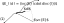
\includegraphics[width=0.25\textwidth]{img/2.png}
    %\caption{}
    %\label{fig:}
\end{figure}

\noindent
Из этих уравнений легко получить, что
\begin{equation}
    \left\{\begin{aligned}
        \frac{\partial U}{\partial z} &= - \frac{L_0}{c^2} \frac{d I}{d t} \\
        \frac{\partial I}{\partial z} &= - C_0 \frac{\partial U}{\partial t} 
    \end{aligned}\right.
    \hspace{0.5cm} \Rightarrow \hspace{0.5cm} 
    \boxed{
        \frac{\partial^2 U}{\partial t^2}  = \frac{c^2}{L_0 C_0} - \frac{\partial^2 V}{\partial z^2} 
    }.
\end{equation}
Решение аналогично будем искать в виде
\begin{equation}
    V = f_1 (z - vt) + f_2 (z + vt),
    \hspace{0.5cm} \Rightarrow \hspace{0.5cm} 
    v = \frac{c}{\sqrt{L_0 C_0}}.
\end{equation}
Кстати, если это всё посчитать для коаксиального кабеля, то
\begin{equation*}
    L_0 = 2 \mu \ln \frac{R_2}{R_1} , \hspace{0.5cm} 
    C_0 = \frac{\varepsilon}{2 \ln \frac{R_2}{R_1} },
    \hspace{0.5cm} \Rightarrow \hspace{0.5cm} 
    v = \frac{c}{\sqrt{\mu \varepsilon}}.
\end{equation*}


\subsubsection*{Коэффициент стоячей волны (standing wave ratio)}
Коэффициент стоячей волны -- отношение наибольшего значения амплитуды напряжённости электрического или магнитного поля стоячей волны в пучностях линии передачи к амплитуде в узлах.
КСВ является мерой согласования нагрузки (например, антенны) с линией передачи.

Наибольшее и наименьшее значения амплитуды соответсвенно равны
\begin{equation*}
    A_{\text{max}} = A_{\text{inc}} + A_{\text{ref}}, \hspace{0.5cm} 
    A_{\text{min}} = A_{\text{inc}} - A_{\text{ref}},
    \hspace{0.5cm} \Rightarrow \hspace{0.5cm} 
    \text{КСВ} = \frac{A_{\text{inc}} + A_{\text{ref}}}{A_{\text{inc}} - A_{\text{ref}}} = 
    \frac{1 + |\Gamma|}{1 - |\Gamma|},
\end{equation*}
где $|\Gamma|$ -- коэффициент отражения.

\subsubsection*{Согласованная нагрузка}
Рассмотрим длинную линию, пусть в цепи 
\begin{equation*}
    U = U_0 \cos \left(\omega_0 t - kz\right),  \hspace{0.5cm} 
    I = I_0 \cos \left(\omega_0 t - kz\right).
\end{equation*}
Сделаем следующий трюк. Возьмем, и продолжим линию до бесконечности, от которой, очевидно, ничего не отразится. Соотвественно нас интересует поиск эквивалентного импеданса системы. 
\begin{align*}
    U^* = U_0 \exp\left(i(\omega_0 t - kz)\right) &= U_0 e^{ikz} e^{-i\omega_0 t}, \\
    I^* = I_0 \exp\left(i(\omega_0 t - kz)\right) &= I_0 e^{ikz} e^{-i\omega_0 t}.
\end{align*}
Подставив эти выражения в волновое уравнение, и получим
\begin{equation*}
    ik U^* = i \omega_0 I^*,
    \hspace{0.5cm} 
    Z^* = U^* / I^* = \frac{\omega_0}{k},
    \hspace{0.5cm} \Rightarrow \hspace{0.5cm} 
    R = \frac{1}{c} \sqrt{\frac{L_0}{C_0}},
    \text{\ \ --- \ \ \textit{согласованная нагрузка}}.
\end{equation*}
То есть при наличии такого сопротивления на конце линии не будет никакого отражения. 




\sbsnum{25}{Формулы гладкой замены переменных в интеграле Лебега от функции}
\subsubsection*{Уравнение непрерывности}
\begin{to_def}[Предмет рассмотрения]
	Ввиду макроскопического рассмотрения \textit{жидкости}(газы) в гидродинамике представлется как сплошная среда, то есть малый элемент объёма жидкости содержит ещё достаточно больше количество молекул, относительно межмолекулярного расстояния.
\end{to_def}

Для описания движения жидкости требуется задать распределение скорости жидкости $\vc{v} = \vc{v}(x,y,z,t)$ и какие-либо её две термодинамические величины, как, например, плотность и давление. Важно отметить, что все эти величины относятся не к отдельной частице, а к точке в пространстве в определенное время.

\begin{to_thr}[Уравнение непрерывности]
\phantom{239}

\begin{proof}[$\triangle$]
	В маленьком объёме $V_{0}$ количество жидкости есть $\int_{V_0} \rho d V$.
	Через элемент поверхности, ограничивающей $V_0$, в единицу времени протекает $\rho \vc{v} \cdot d \vc{f}$ жидкости --- положительно или отрицательное число, в зависимости от того, вытекает или втекает жидкость соответственно.
	Тогда приравниваем для вытекания жидкости два наших рассуждения:
	\begin{equation*}
		- \frac{\partial}{\partial t} \int \rho d V =  \oint \rho \vc{v} \cdot d \vc{f}
		\hspace*{0.5 cm} 
		\Rightarrow 
		\hspace*{0.5 cm}
		\int \left(\frac{\partial \rho}{\partial t} + \div \rho \vc{v}\right)d V = 0
		\hspace*{0.5 cm}
		\Rightarrow
		\hspace*{0.5 cm}
		\frac{\partial \rho}{\partial t} + \div \rho \vc{v} = 0.
	\end{equation*}
	Последнее следует из того, что равенство должно иметь для любого объёма, таким образом получили искомое \textit{уравнение непрерывности}.
\end{proof}
	
\end{to_thr}

\subsubsection*{Уравнение Эйлера}

\begin{to_thr}[Уравнение Эйлера]
\phantom{239}

\begin{proof}[$\triangle$]
	Выделим в жидкости некоторый объём, полная сила, действующая на этот объём: $- \oint p d \vc{f} = - \int \grad p d V$, где интеграл из взятого по поверхности объёма преобразуется в сам рассматриваемый объём.
	Таким образом получили, что на единицу объёма жидкости будет действовать сила:
	\begin{equation*}
		\rho \frac{d \vc{v}}{d t} = - \grad p.
	\end{equation*}
	Однако стоящая здесь скорость определяет изменение скорости именно элемента объёма, а не точки в пространстве.
	Запишем это изменение скорости:
	\begin{equation*}
		d \vc{v} 
		=
		 \frac{\partial \vc{v}}{\partial t} d t + \frac{\partial \vc{v}}{\partial x^i} d x^i 
		= 
		\frac{\partial \vc{v}}{\partial t} d t + (d \vc{r} \cdot \nabla) \vc{v}
		\hspace*{1 cm}
		\Rightarrow
		\hspace*{1 cm}
		\frac{\partial \vc{v}}{\partial t} + (\vc{v} \nabla) \vc{v} = - \frac{1}{\rho} \grad p.
	\end{equation*}
	Последнее и есть искомое уравнение Эйлера.
\end{proof}
\end{to_thr}

Если же жидкость движется во внешнем поле тяжести, то, на каждый элемент объёма будет действовать сила, которая просто добавится к изначальному уравнению: 
\begin{equation*}
	\frac{\partial \vc{v}}{\partial t} + (\vc{v} \nabla) \vc{v} = - \frac{\nabla p}{\rho} + \vc{g}.
\end{equation*}

\subsubsection*{Уравнение Навье-Стокса}

Чтобы нормально учесть вязкость, нужно поговорить про \textit{поток импульса}.
Импульс единицы объёма жидкости есть $\rho \vc{v}$, скорость изменения его компоненты:
\begin{equation*}
	\frac{\partial}{\partial t} \rho v^i = \rho \frac{\partial v^i}{\partial t} + \frac{\partial \rho}{\partial t} v^i.
\end{equation*}
Уравнения непрерывности и Эйлера запишутся в тензорном виде:
\begin{equation*}
	\frac{\partial \rho}{\partial t} = - \frac{\partial (\rho v^k)}{\partial x^k},
	\hspace*{0.5 cm}
	\hspace*{0.5 cm}
	\frac{\partial v^i}{\partial t} = - v^k \frac{\partial v^i}{\partial x^k} - \frac{1}{\rho} \delta^{i k} \frac{\partial p}{\partial x^k}.
\end{equation*}
Тогда получим:
\begin{equation*}
	\frac{\partial}{\partial t} \rho v^i 
	= 
	- \rho v^k \frac{\partial v^i}{\partial x^k} -  \delta^{i k} \frac{\partial p}{\partial x^k} - v^i \frac{\partial \rho v^k}{\partial x^k} 
	=
	-\delta^{i k} \frac{\partial p}{\partial x^k} - \frac{\partial}{\partial x^k} \rho v^i v^k
	= - \frac{\partial \Pi^{i k}}{\partial x^k}.
\end{equation*}
\begin{to_def}
	$\Pi^{i k} $ --- \textit{тензор плотности потока импульса}:
	$
		\Pi^{i k} = p \delta^{i k} + \rho v^i v^k.
	$
\end{to_def}

Таким образом уравнение Эйлера у нас записалось в виде:
$
	\frac{\partial}{\partial t} \rho v^i = - \frac{\partial \Pi^{i k}}{\partial x^k}.
$
Поток импульса представляет собой чисто обратимый перенос импульса, связанный с просто механическим передвижением различных участков жидкости и с действующими в жидкости силами давления.
\textit{Вязкость} (внутреннее трение) жидкости проявляется в наличии ещё дополнительного, необратимого переноса импульса из мест с большой скоростью в места с меньшей.

Поэтому уравнение движения вязкой жидкости можно получить, прибавив к идеальному потоку импульса дополнительный член $\sigma^{i k}_{visc}$, определяющий такой вязкий перенос:
$
\Pi^{i k} = p \delta^{i k} + \rho v^i v^k - \sigma^{i k}_{visc} = - \sigma^{i k} + \rho v^i v^k.
$
\begin{to_def}
	Таким образом: $\sigma^{i k} = - p \delta^{i k} + \sigma^{i k}_{visc}$ называют \textit{тензором напряжений}, а $\sigma^{i k}_{visc}$ --- вязким тензором напряжений.
\end{to_def}

Чтобы написать выражение для вязкого напряжения сделаем пару оговорок. 
\textit{Во первых}, градиенты скорости движения участков жидкости относительно друг друга не велики, тогда $\sigma^{i k}_{visc}$ зависит лишь от первых производных скорости по координатам, линейно. \textit{Во вторых}, не зависящие от первых производных величины должны обращаться в нуль как для скорости потока $\vc{v} = \const$ и тензор должен быть нулевым. \textit{В третьих}, $\sigma^{i k}_{visc} = 0$ когда жидкость совершает целое равномерное вращение, поскольку никакого внутреннего трения тогда не будет.
Для такого равномерного вращения с $\vc{v} = [\vc{\omega} \vc{r}]$ линейными комбинациями производных обращающимися в нуль будут: $\frac{\partial v^i}{\partial x^k} + \frac{\partial v^k}{\partial x^i}$.

Это всё даёт нам мотивацию для не шибко сильных потоков несжимаемой жидкости согласится с Сэром Исааком Ньютоном, и написать тензор вязкого напряжения, как \textit{тензор скорости деформации}:
\begin{equation*}
	\sigma^{i k}_{visc} = \eta \left(\frac{\partial v^i}{\partial x^k} + \frac{\partial v^k}{\partial x^i}\right),
	\hspace*{1 cm}
	\Rightarrow
	\hspace*{1 cm}
	\sigma^{i k} = - p \delta^{i k} + \eta \left(\frac{\partial v^i}{\partial x^k} + \frac{\partial v^k}{\partial x^i}\right).
\end{equation*}
А уравнение Эйлера тогда для несжимаемой жидкости запишется:
\begin{equation*}
	\rho \left(\frac{\partial v^i}{\partial t} + v^k \frac{\partial v^i}{\partial x^k}\right)
	=
	- \delta^{i k} \frac{\partial p}{\partial x^k} + \frac{\partial}{\partial x^k} \left[\eta \left(\frac{\partial v^i}{\partial x^k} + \frac{\partial v^k}{\partial x^i}\right)\right].
\end{equation*}
а в более человеческом, привычном глазу, виде \textit{уравнение Навье-Стокса для несжимаемой жидкости}:
\begin{equation*}
	\frac{\partial \vc{v}}{\partial t} + (\vc{v} \triangle) \vc{v} = - \frac{1}{\rho} \grad p + \frac{\eta}{\rho} \Delta \vc{v}.
\end{equation*}
\begin{to_def}
	Коэффициент $\eta$ называется --- \textit{динамическим коэффициентом вязкости}, а отношение $\eta/\rho = \nu$ --- \textit{кинематической вязкостью}.
\end{to_def}


\newpage 

\sbsnum{7}{Теорема о расщеплении гладкого отображения}
\sbsnum{26}{Вложенные многообразия}
Напишем систему уравнений, соответствующую уравнениям Лагранжа первого рода:

\begin{equation}
    \sum_{\nu=1}^N \vc{a}_{\beta \nu} (\vc{r}_1, \ldots, \vc{r}_N, t) \cdot \vc{v}_\nu + a_\beta  (\vc{r}_1, \ldots, \vc{r}_N, t) = 0,
    \hspace{0.5cm} (\beta = 1, \ldots, s)
\end{equation}
$$
    f_\alpha (\vc{r}, t) = 0, \hspace{0.5cm} (\alpha = 1, \ldots, r),
$$
\begin{align}
    \sum_{\nu=1}^N \frac{\partial f_\alpha}{\partial \vc{r}_\nu} \cdot d \vc{r}_\nu + \frac{\partial f_\alpha}{\partial t} d t &= 0,
    \hspace{0.5cm} &(\alpha = 1, \ldots, r), \\
    \sum_{\nu=1}^N \vc{a}_{\beta\nu} \cdot d \vc{r}_\nu + a_\beta d t &= 0,
    \hspace{0.5cm} &(\beta = 1, \ldots, s).
\end{align}



Взяв выражения для виртуальных перемещений всегда можно получить силы реакции так называемым методом \textit{множителей Лагранжа}:
\begin{equation*}
    \sum_{\nu=1}^N \left(\vc{R}_\nu - \sum_{i = 1}^r \lambda_i \frac{\partial f_i}{\partial \vc{r}_\nu} - \sum_{j = 1}^s \mu_j \alpha_{j \nu}\right) \delta \vc{r}_\nu = 0
    \hspace*{1 cm}
    \Rightarrow
    \hspace*{1 cm}
    \vc{R}_\nu = \sum_{i = 1}^r \lambda_i \frac{\partial f_i}{\partial \vc{r}_\nu} + \sum_{j = 1}^s \mu_j \alpha_{j \nu}.
\end{equation*}
Полученные выражения для реакций идеальных сил через неопределенные множители Лагранжа $\lambda_i $ и $\mu_j $ можно подставить в исходное уравнение связей, получим \textit{уравнения Лагранжа первого рода}:
\begin{equation*}
    m_\nu \vc{w}_\nu = \vc{F}_\nu + \sum_{i = 1}^r \lambda_i \frac{\partial f_i}{\partial \vc{r}_\nu} + \sum_{j = 1}^s \mu_j \alpha_{j \nu}.
\end{equation*}

\sbsnum{27}{* Абстрактное определение гладкого многообразия}
\subsubsection*{Преломление и поглощение волн}

Пусть есть некоторое внешнее поле $E = E_0 e^{i(\omega t - kz)}$. Посмотрим на электрон на орбите атома,
\begin{equation*}
    m \ddot{z} = - k z - \beta \dot{z} + E_0 \cdot e^{-i(\omega t - kz)},
    \hspace{0.5cm} \overset{p = e z}{\Rightarrow}  \hspace{0.5cm} 
    \ddot{p} + 2 \delta \dot{p} + \omega_0^2 p = \frac{eE_0}{m} e^{-i(\omega t - kz)},
\end{equation*}
будем искать решения вида $p = p_0 e^{i\omega t}$, тогда
\begin{equation*}
    p = \frac{eE_0}{m} \frac{
    1
    }{
    (\omega_0^2 - \omega_2) - 2 \delta \omega i 
    } 
    e^{-i(\omega t - kz)}.
\end{equation*}
Вспомним, что $D$ равно
\begin{equation*}
     D = E + 4 \pi N p = 
     \bigg(
     \underbrace{
     1 + \frac{4\pi N e^2}{m} \cdot 
     \frac{1}{(\omega_0^2 - \omega^2) - 2 \delta \omega i} 
     }_{\varepsilon}
    \bigg) E.
\end{equation*}
По определению $n = \sqrt{\varepsilon}$, то есть
\begin{equation*}
    n^2 = \varepsilon = 1 + \frac{4\pi N e^2}{m} \cdot 
     \frac{1}{(\omega_0^2 - \omega^2) - 2 \delta \omega i}.
\end{equation*}

В случае проводника $\omega_0 = 0$, к тому же $2 \delta = 1 / \tau$, где $\tau$ -- характерное время затухания. Запишем, что
\begin{equation*}
    j = \sigma E, \hspace{0.5cm} j = N e v,
    \hspace{0.5cm} 
    v = \frac{eM}{m} \tau
    \hspace{0.5cm} \Rightarrow \hspace{0.5cm} 
    \tau = \frac{m\sigma}{Ne^2}. 
\end{equation*}
Тогда для проводника
\begin{equation*}
    n^2 = 1 - \frac{4\pi\sigma}{\omega i (1 -i \omega \tau)}.
\end{equation*}
Рассмотрим два случая, когда $\omega \tau \ll 1$, и $\omega \tau \gg 1$. 

\subsubsection*{Скин-эффект}


Первый случай приводит нас к явлению скин-эффекта.
\begin{equation*}
    n^2 = 1 - \frac{4\pi\sigma}{\omega i (1 -i \omega \tau)} 
    \approx
    1 - \frac{4\pi \sigma}{\omega i} \approx i \frac{4 \pi \sigma}{\omega},
    \hspace{0.5cm} \Rightarrow \hspace{0.5cm} 
    n = \left(\frac{1 + i}{\sqrt{2}}\right) \sqrt{\frac{4\pi\sigma}{\omega}}
    = \sqrt{\frac{2\pi\sigma}{\omega} } (1 + i)
    .
\end{equation*}
Посмотрим к чему это приводит. 
\begin{equation*}
    E = E_0 e^{-i(\omega t - kz)}, \hspace{0.5cm} 
    k = \frac{\omega}{c} \sqrt{\varepsilon \mu} = \frac{\omega}{c} n.
\end{equation*}
Тогда
\begin{equation*}
    E = E_0 e^{-i(\omega t - \frac{n}{c} z)} = E_0
    e^{-i \omega t} \exp\left(
        i \frac{\omega}{c} \sqrt{\frac{2\pi\sigma}{\omega} }z
    \right)
    \exp\left(
        - \frac{\omega}{c} \sqrt{\frac{2\pi\sigma}{\omega} }
    \right).
\end{equation*}
Появился множитель, соответсвующий экспоненциальному затуханию
\begin{equation*}
    z_0 = \sqrt{\frac{c^2}{2\pi \sigma \omega} },
\end{equation*}
где на $z_0$ происходит затухание в $e$ раз. 


\subsubsection*{Прозрачность металлов}

Первый случай приводит к прозрачности металлов.
\begin{equation*}
    n^2 = 1 - \frac{4\pi\sigma}{\omega i (1 -i \omega \tau)} 
    \approx
    1 - \frac{4\pi\sigma}{\omega^2 \tau} = 1 - \frac{\omega_{\text{p}}^2}{\omega^2} 
    ,
    \omega_{\text{p}}:2 = 
    \frac{4 \pi \sigma}{\tau} = \frac{4 \pi N e^2}{m}.
\end{equation*}
То есть при $\omega < \omega_{\text{p}}$ происходит отражение, а при $\omega > \omega_{\text{p}}$ металл становится прозрачным, то есть похожим на диэлектрик. 






% \subsubsection*{Бонус о плазме}







\sbsnum{28}{Диф-формы, векторные поля и \texorpdfstring{$d$}{d} на многообразии}

Легко получить соотношение вида
\begin{equation}
    \sum_{i=1}^N \left(
        \vc{F}_i - m_i \vc{\mathrm{w}}_i
    \right) \cdot \delta \vc{r}_i = 0.
\end{equation}
Данное соотношение является необходимым и достаточным условием для того, чтобы движение, совместимое с идеальными связями, отвечало данной системе активных сил $\vc{F}_i$. Оно получило название \textbf{общего уравнения динамики} или \textit{дифференциальным вариационным принципом Даламбера-Лагранжа}.

\begin{to_thr} [принцип Даламбера-Лагранжа]
Верно, что
\begin{equation*}
    m_i \vc{\mathrm{w}}_i = \vc{F}_i + \vc{R}_i,
    \hspace{0.5cm} \Rightarrow \hspace{0.5cm} 
    \sum_i \left(
       \vc{F}_i -  m_i \vc{\mathrm{w}}_i
    \right) \cdot \delta \vc{r}_i = 0.
\end{equation*}
\end{to_thr}

Аналогично можно сформулировать \textit{принцип Журдена}
\begin{equation}
    \sum_{i=1}^N \left(
        \vc{F}_i - m_q \vc{\mathrm{w}}_i
    \right) \cdot \delta  \vc{v}_i = 0,
\end{equation}
и \textit{принцип Гаусса}:
\begin{equation}
    \sum_{i=1}^N \left(
        \vc{F}_i - m_q \vc{\mathrm{w}}_i
    \right) \cdot \delta \vc{\mathrm{w}}_i = 0,
\end{equation}
где $\delta \vc{\mathrm{w}}_i = \vc{\mathrm{w}}^*_{i_1} - \vc{\mathrm{w}}^*_{i_2}$ не обязательно малая величина. 

Замечая, что $m_i = \const$, а $\vc{F}_i = \vc{F}_i (p, q)$, то последнее уравнение перепишется в виде
\begin{equation*}
    Z = \frac{1}{2} \sum_{i=1}^N m_i 
    \left(
        \vc{\mathrm{w}}_i - \frac{\vc{F}_i}{m_i} 
    \right)^2,
    \hspace{1cm} 
    \delta Z = 0,
\end{equation*}
где величина $Z$ называется принуждением или мерой принуждения. К слову она не просто стационарна для истинных движений. 

\texttt{Истинным является движение с минимальной мерой принуждения.} Другими словами \textit{несвободная система совершает движение, наиболее близкое к свободному}. 

\begin{to_def} 
    Будем считать, что $q^0 \in M$ -- \textit{точка равновесия}, если при $\dot{q}^0 \equiv \dot{q}(0) \equiv 0$ приводит к $q(t) = q^0$. 
\end{to_def}

В таком случае верен следующий принцип:

\begin{to_thr}[принцип Лагранжа]
    Для того, чтобы точка была положением равновесия на $t \in [t_1, t_2]$ необходимо и достаточно, чтобы сумма элементарных работ на $\forall$ виртуальных перемещениях всех активных сил была равна нулю.
    \begin{equation}
        \delta A \big|_0 = 0 
        \hspace{0.5cm} 
        \delta A = \sum_i \vc{F}_i \cdot \delta \vc{r}_i,
        \hspace{0.5cm} (t\in[t_1, t_2])
    \end{equation}
    что является \textbf{общим уравнением статики}.
\end{to_thr}

Этот принцип можно рассматривать, как дракона с тремя головами. Вот если система \textbf{голономная}, то
\begin{equation*}
    \delta A = Q_i \delta q_i 
    \hspace{0.5cm} \Rightarrow \hspace{0.5cm} 
    Q_i = 0 \ \forall i.
\end{equation*}
Если система \textbf{консервативная}, то
\begin{equation*}
    Q_1 = - \frac{\partial P}{\partial q^i} 
    \hspace{0.5cm} \Rightarrow \hspace{0.5cm} 
    \text{положение равновесия --- стационарная точка потенциала}.
\end{equation*}
Если же у нас \textbf{твёрдое тело}, тогда
\begin{equation*}
    \delta A = \left(
        \vc{R}^{\text{внеш}} \cdot \vc{v}_O
    \right) \d t + 
    \left(
        \vc{M}_O^{\text{внеш}} \cdot \vc{\omega}
    \right) dt
    \hspace{0.5cm} \Rightarrow \hspace{0.5cm} 
    \left\{\begin{aligned}
        \vc{R}^{\text{внеш}} &= 0 \\
        \vc{M}^{\text{внеш}} &= 0 \\
    \end{aligned}\right.
\end{equation*}



\sbsnum{29}{Гладкие отображения многообразий}

\begin{to_def} 
    Функция $f \colon M \mapsto \mathbb{R}$ называется \textit{гладкой функцией на многообразии}, $f \in C^{\infty}(M)$, если в каждой координатной карте $\varphi \colon U \mapsto \mathbb{R}^n$ эта функция ($f \circ \varphi^{-1}$) является гладкой функцией на образе $\varphi(U)$.
\end{to_def}



\begin{to_def} 
    \textit{Гладкой структурой} на топологическом пространстве называется максимальный по включению атлас, с которым пространство становится многообразием. 
\end{to_def}


\begin{to_def} 
    \textit{Гладким отображением} между многообразиями $f \colon M \mapsto N$ размерностей $m$ и $n$ называется непрерывное отображение, которое в окрестности каждой точки, в достаточно малых координатных картах, выглядит как гладкое отображение из $\mathbb{R}^m$ в $\mathbb{R}^n$.
\end{to_def}


\begin{to_def} 
    Гладкое обратимое отображение $f \colon M \mapsto N$ с обратным гладким назовётся \textit{диффеоморфизмом многообразий}. 
\end{to_def}

\begin{to_tas} 
\label{task_6.131} % + текст с 227 страницы.
    Если взять некоторое \textit{компактное} гладкое многообразие $M$ (область параметров) и гладкое отображение $f \colon M \mapsto \mathbb{R}^n$, такое, что $\rg Df_p = \dim M$ $\forall p$, то $f(M)$ будет вложенным многообразием.     
\end{to_tas}

\begin{to_lem} 
    Для гладкого отображения $f \colon M \mapsto \mathbb{R}^n$ с $\rg Df \equiv m = \dim M$, для всякой $p \in M$ найдётся окрестность $U \ni p$ такая, что $f(U)$ в некоторой криволинейной системе координат в окрестности $f(p)$ является открытым подмножеством стандартно вложенного $\mathbb{R}^m \subseteq \mathbb{R}^n$. 
\end{to_lem}


\sbsnum{30}{Ориентируемость многообразия}
\begin{to_def} 
    Гладкое многообразие $M$ называется \textit{ориентируемым}, если можно выбрать покрывающий атлас так, что якобианы замен координат между любыми двумя картами атласа будут положительными. 
\end{to_def}

Если в исходном атласе был задан некоторый объект, например векторное поле $X$, то во всякой новой карте $\psi$ мы тоже будем иметь векторное поле, собранное из прямых образов $(\psi  \circ \varphi^{-1})_* X_\varphi$ полученных с имеющихся карт $\varphi$ и образов $X_\varphi$ в них.

\begin{to_def} 
    \textit{Ориентацией гладкого многообразия} $M$ называется атлас с положительными якобианами перехода между картами, максимальный по включению среди всех таких атласов. 
\end{to_def}

\begin{to_lem} 
    Связное многообразие либо неориентируемо, либо допускает два класса ориентации. 
\end{to_lem}

\begin{to_lem} 
    Многообразие $M$ размерности $n$ ориентируемо тогда и только тогда, когда существует дифференциальная форма $\nu \in \Omega^n (M)$, которая ни в одной точку не равна нулю.
\end{to_lem}

\begin{to_lem} 
\label{zorich_cXV.p2.lem4} % см. страницу 308
    Многообразие ориентируемо тогда и только тогда, когда на нём не существует противоречивой (дезориентирующей) цепочки карт.
\end{to_lem}

\begin{to_def} 
    Для $n$-мерного ориентированного многообразия с краем $M$ введём ориентацию на его крае $\partial M$ следующим образом. Пусть карта $M$ с координатами $x_1, \ldots, x_n$ соответсвует ориентации $M$, причём образ отображения карты удовлетворяет неравенству $x_1 \leq 0$, а образ края соответствует равенству $x_1 = 0$. Тогда карта на соответствующей части $\partial M$ из координат $x_2, \ldots, x_n$ по определению объявляется положительной. Если же многообразие в этой карте задано неравенством в другую сторону, $x_1 \geq 0$, то карта $x_2, \ldots, x_n$ на его краю по определению объявляется отрицательной. 
\end{to_def}

\begin{to_lem} 
    Предыдущее определение корректно задаёт ориентацию на $\partial M$. 
\end{to_lem}








\sbsnum{31}{Определение интеграла диф-формы по ориентированному многообразию}
\begin{to_lem}[Разбиение единицы в окрестности компакта на многообразии]
     Пусть $M$ -- гладкое многообразие, а $K \subseteq M$ -- его компактное подмножество. Для любого покрытия $\{U_\alpha\}_\alpha$ компакта $K$ открытыми множествами найдётся набор неотрицательных гладких функций $\{\rho_\alpha\}_\alpha$ с компактными носителями $\mathrm{supp}\, \rho_\alpha$ таких, что
\begin{equation*}
    \forall \alpha \ \textnormal{supp}\, \rho_\alpha \subset U_\alpha,
\end{equation*}
    только конечное число из них отлично от нуля и
    $\sum_\alpha \rho_\alpha (x) \equiv 1$
    в некоторой окрестности $K$.
\end{to_lem}

\begin{to_def} 
    Интеграл дифференциальной формы $\nu \in \Omega_{\text{c}}^n (M)$ с компактным носителем по ориентированному $n$-мерному многообразию $M$ определяется с помощью разбиения единицы в окрестности носителя $\nu$ 
    \begin{equation*}
         \rho_1 + \ldots + \rho_m = 1,
     \end{equation*} 
     подчиненного некоторому набору положительно ориентрированных карт как
     \begin{equation*}
         \int_M \nu = \sum_i \int_M \rho_i \nu_i,
     \end{equation*}
     где интегралы справа рассматриваются в координатных картах, содержащих носители соответствующих $\rho_i$.
\end{to_def}

\begin{to_lem} 
    Определение интеграла не зависит от выбора системы положительных карт в данной ориентации и подчиненного им разбиения единциы. 
\end{to_lem}





\sbsnum{32}{Общая формула Стокса} 
Подставим разложение кинетической энергии в уравнения Лагранжа, оставив только слагаемые с обобщёнными ускорениями $f_j (q, \dot{q}, t) = a_{jk} \ddot{q}^j$. 
\begin{equation*}
    T = \frac{1}{2} \sum_\nu m_\nu \dot{\vc{r}}_\nu^2 = \frac{1}{2} \sum_\nu
    \left(
        \frac{\partial \vc{r}_\nu}{\partial q^j} \dot{q}^j + \frac{\partial \vc{r}_\nu}{\partial t} 
    \right)^2 = 
    \frac{1}{2} 
    \bigg[
    \underbrace{
        a_{jk} \dot{q}^j \dot{q}^k
    }_{
        2T_2
    } +
    \underbrace{
        a_j \dot{q}^j
    }_{
        2T_1
    } +
    \underbrace{
        a_0
    }_{
        2T_0
    }
    \bigg],
\end{equation*}
где коэффициенты, соответственно, равны 
\begin{equation*}
    a_{jk}(q, t) = \sum_\nu m_\nu \frac{\partial \vc{r}_\nu}{\partial q^j} \cdot \frac{\partial \vc{r}_\nu}{\partial q^k},
    \hspace{0.5cm} 
    a_j(q, t) = \sum_\nu m_\nu \frac{\partial \vc{r}_\nu}{\partial q^j} \cdot \frac{\partial \vc{r}_\nu}{\partial t},
    \hspace{0.5cm} 
    a_0 = \sum_\nu m_\nu 
    \left(
    \frac{\partial \vc{r}_\nu}{\partial t} 
            \right)^2.
\end{equation*}
Для склерономных систем $\partial \vc{r}_\nu / \partial t = 0$, соотвественно $T = a_{jk} \dot{q}^j \dot{q}^k$, при чём $a_{jk} \equiv a_{jk} (q)$.

Теперь подставим значение $T$ в уравнения Лагранжа, и получим, что
$
    a_{ik} \ddot{q}^k = f_i,
$
где $f_1 = f_1(q, \dot{q}, t)$. Уравнений в системе $n$, причём $a_{jk}$ является положительно определенной формой\footnote{
    \red{Требует отдельного доказательства.}
}, соответственно невырожденной. 

\begin{to_thr} 
    Уравнения Лагранжа второго рода разрешимы относительно обобщенных ускорений 
\end{to_thr}
 

\sbsnum{33}{Частные случаи формулы Стокса}
 % \renewcommand{\labelenumi}{\Roman{enumii}}
\begin{enumerate}[label={$\mathbb{R}^\text{\arabic*}$.}]
    \item Формула Стокса для ориентированной кривой с началом в точке $p$ и концом в точке $q$ сводится к 
    \begin{equation*}
        \int_\gamma \d f = f(q) - f(p).
    \end{equation*}
    \item Для компактного множества $G \subset \mathbb{R}^2$ с гладкой границей, ориентированного так, что при движении по $\partial G$ множество $G$ оказывается слева, верна \textit{формула Грина}
    \begin{equation*}
        \int_{\partial G} P \d x + Q \d y = \int_G
        \left(
            \frac{\partial Q}{\partial x} - \frac{\partial P}{\partial y} 
        \right) \d x \wedge d y.
    \end{equation*}
    \item Для компактного множества $G \subset \mathbb{R}^3$ с гладкой границей (край в $\mathbb{R}^3$) верна \textit{формула Гаусса-Остроградского}
    \begin{equation*}
        \int_{\partial G} P \d y \wedge d z 
        + Q \d z \wedge dx 
        + R \d x \wedge dy = 
        \int_G
        \left(
            \frac{\partial P}{\partial x} +
            \frac{\partial Q}{\partial y} +
            \frac{\partial R}{\partial z} 
        \right) \d x \wedge d y \wedge d z.
    \end{equation*}
\end{enumerate}


Кривую можно считать не бесконечно гладкой, а всего лишь кусочно непрерывно дифференцируемой, формула всё равно остаётся верной. С помощью предельного перехода также обобщается случай с $\simeq \mathbb{R}^2$ до множества с кусочно $C^2$ границей.

Вообще формула Стокса верна не только для вложенных двумерных многообразий, но и для всякого образа гладкого отображения $f \colon D \mapsto  \mathbb{R}^3$ области $D \subset \mathbb{R}^2$ с кусочно гладкой границей, если интегралы мы понимаем как интегралы обратных образов $f^*(\alpha)$ и $f^*(d\alpha)$ по $\partial D$ и $D$ соответственно. Для практических применений полезно ослабить условие гладкости $f$ до $C^2$ (в интеграле, в координатном представлении, используются производные $f$ не более чем первого порядка).


% Кривую 

 % дописать материал из Зорича

\sbsnum{34}{Потенциал диф-форм}
Физический потенциал силового поля в математический терминах означает поиск $f \in C^\infty (M) \colon \d f = \alpha$ для заданной силы $\alpha \in \Omega^1(M)$

\begin{to_thr}
	Необходимым и достаточным условием наличия потенциала у непрерывной $\alpha \in \Omega^1(M)$, для гладкого $M$, является независимость $\int_\gamma \alpha$ от выбора между двумя точками кусочно-гладкой кривой $\gamma$.

	Эквивалентно можно потребовать равенства нулю интегралов по всем замкнутым кусочно-гладким кривым.
	\label{thr_7.1}
\end{to_thr}

Удобным на практике необходимым условием существования потенциала у $\alpha \in \Omega^1(M)$ является $\d \alpha = 0$ (т.к. $\d (\d u) = 0$).
Однако этого не достаточно, так например в открытой $U = \mathbb{R}^2 \backslash \{ 0 \}$:
\begin{equation*}
	\alpha = \frac{x \d y - y \d x}{x^2 + y^2}
	\hspace*{0.5 cm} \leadsto \hspace*{0.5 cm}
	\d \alpha = 0,
	\hspace*{0.5 cm} \text{ но } \hspace*{0.5 cm}
	\oint_{S^1} \alpha = 2 \pi.
\end{equation*}

Далее в качестве упражнений оставлены следующие важные замечания:

\begin{to_tas}[Порядок точки относительно кривой]
Для замкнутой кусочно-гладкой $\gamma \in \mathbb{R}^2$, не проходящей через начало координат определим порядок начала координат относительно кривой:
\begin{equation*}
	w (\gamma, 0) - \frac{1}{2 \pi} \int_{\gamma} \frac{x \d y - y \d x}{x^2 + y^2},
\end{equation*}
и он не меняется при непрерывных деформациях кривой, при которых она не проходит через начало координат.
\end{to_tas}

\begin{to_tas}
	Порядок начала координат относительно кривой является целым.
\end{to_tas}

\begin{to_tas}
	Порядок начала координат относительно не проходящей через него нечётной кривой является нечётным числом. ($\gamma \colon \mathbb{S}^1 \rightarrow \mathbb{R}^2, \; \gamma(-u) = - \gamma(u)$).
\end{to_tas}

\begin{to_tas}
	Для замкнутой кривой на плоскости с всюду не нулевой скоростью $\int k(s) \d s = 2 \pi N, \; N \in \mathbb{Z}$.
\end{to_tas}

\begin{to_tas}[Лемма Жордана]
	Замкнутая кусочно-гладкая кривая $\gamma \subset \mathbb{R}^2$ без самопересечений делит плоскость на две связные части внутреннюю и внешнюю (можно усложнить и сформулировать для непрерывных кривых).
\end{to_tas} % дописать материал из Зорича

\newpage 


\section*{Векторы и дифференциальны формы первой степени}

\sbsnum{13}{Вектор, как дифференцирование}


% 6.6. Векторы и векторные поля

\begin{to_lem} 
    % 6.44
    Всякую гладкую функцию, определенную в некоторой окрестности $x_0 \in \mathbb{R}^n$, в возмоно меньшей окрестности $x_0$, можно представить в виде
    \begin{equation*}
         f(x) = f(x_0) + \sum_{k=1}^n (x_k  - x_{0, k}) g_k (x), 
     \end{equation*} 
     с гладкими $g_k$.
\end{to_lem}
% \newpage 





% \input
% \input

